\documentclass{standalone}

%colors
\usepackage[dvipsnames]{xcolor}

% tikz
\usepackage{tikz}
\usetikzlibrary{positioning,fit,shapes,decorations.pathreplacing}
%\usepackage{tikz-3dplot}

\newcommand*{\xMin}{1}%
\newcommand*{\xMax}{8}%
\newcommand*{\yMin}{1}%
\newcommand*{\yMax}{4}%

\begin{document}
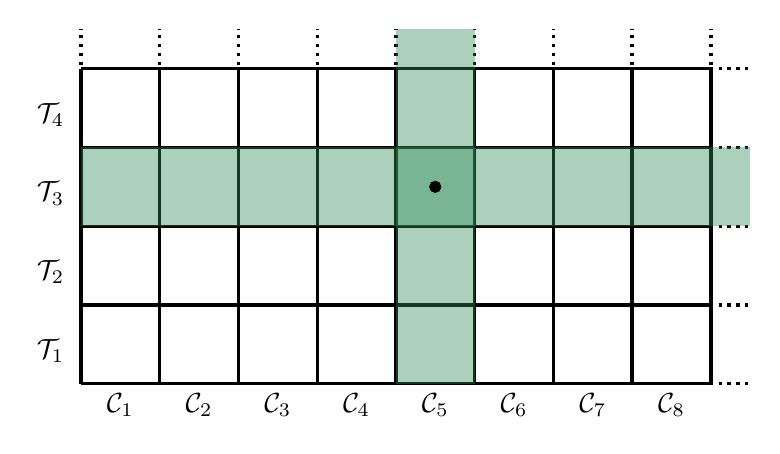
\begin{tikzpicture}
    \foreach \i in {\xMin,...,\xMax} {
        \draw node [below] at (\i-0.5,\yMin-1) {$\mathcal{C}_{\i}$};
    }
    %%\draw node [below] at (\xMax+0.5,\yMin-1.1) {$\dots$};
    \foreach \i in {\yMin,...,\yMax} {
        \draw node at (\xMin-1,\i-0.2,) {$\mathcal{T}_{\i}$};
    %\draw node at (\xMin-1,\yMax+0.8,) {$\vdots$};
    }
        \draw [step=1.0, black, very thick] (0.0,0.0) grid (\xMax,\yMax);
        %\node at (2.5,1.5) {\footnotesize{$(C, T)$}};
        \draw [step=1.0, black, very thick, dotted] (0.0,0.0) grid (\xMax+0.5,\yMax+0.5);
        
        \fill [SeaGreen, opacity=0.4] (4,0) rectangle (5, \yMax+0.5);
        \fill [SeaGreen, opacity=0.4] (0,2) rectangle (\xMax+0.5, 3);

        \filldraw [black] (4.5,2.5) circle (2pt);
\end{tikzpicture}
\end{document}